\section{Techniken}

\subsection{Personendaten}
\frame{\frametitle{Personendaten}

Weit verbreitet zur Verwaltung von Personendaten sind \textbf{Directories}. Diese können über \textbf{DSML}\footnote{Directory Services Markup Language}, einer auf XML basierten Sprache angesprochen werden und ermöglicht somit Applikationen Daten aus den Directories zu lesen oder in die Directories zu schreiben.\\[2ex]

Eine Alternative wäre die Nutzung eines relationalen Datenbanksystem.

}

\subsection{Authentisierung}
\frame{\frametitle{Authentisierung}

Der Anwender muss

\begin{itemize}
\item etwas wissen,
\item etwas besitzen oder
\item etwas sein.
\end{itemize}

	Weitere Techniken, welche bei der Authentisierung verwendet werden sind: \textbf{SASL}, \textbf{TLS} und \textbf{SSO Systeme}.
}

\subsection{Autorisierung}
\frame{\frametitle{Autorisierung}
Um die Verteilung von Rechten und Rollen zu steuern gibt es technisch nicht viele Möglichkeiten.

\begin{itemize}
\item Eingabemaske
\item Workflow
\item Regeln
\end{itemize}
}

\frame{\frametitle{XACML}
\begin{center}
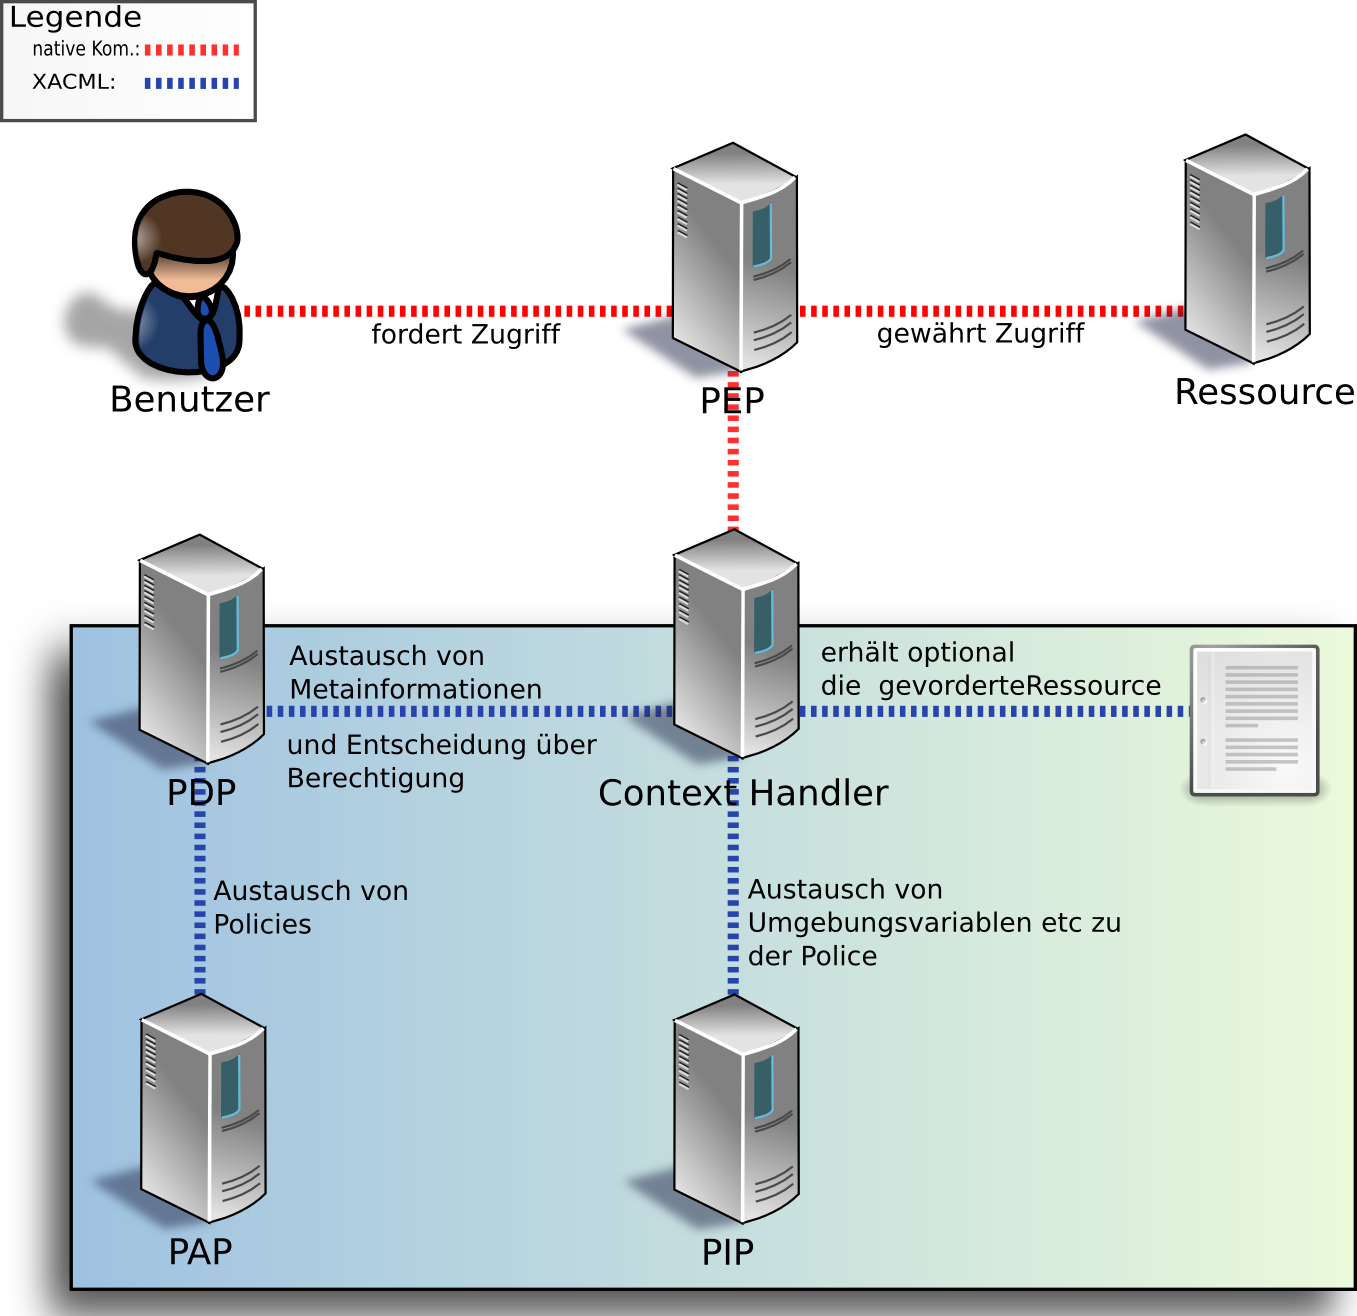
\includegraphics[scale=0.4]{pic/XACML}
\end{center}
}